\chapter{Implementación}

En este capítulo se explicará las implementaciones realizadas para poder llevar a cabo el proyecto, tanto como para conseguir la comunicación con el sensor, los cambios realizados en Aaaida para poder visualizar las mediciones del sensor y por último el despliegue en la Raspberry Pi. 

\section{Comunicación con el sensor}

Para la realización del proyecto es necesario un sensor que se pueda comunicar y enviar los datos mediante bluetooth. En la empresa se dispone de una serie de sensores médicos de los cuales se utilizará un monitor de ritmo cardiaco, Zephyr BioHarness 3. 

\begin{figure}[htb]
\begin{center}
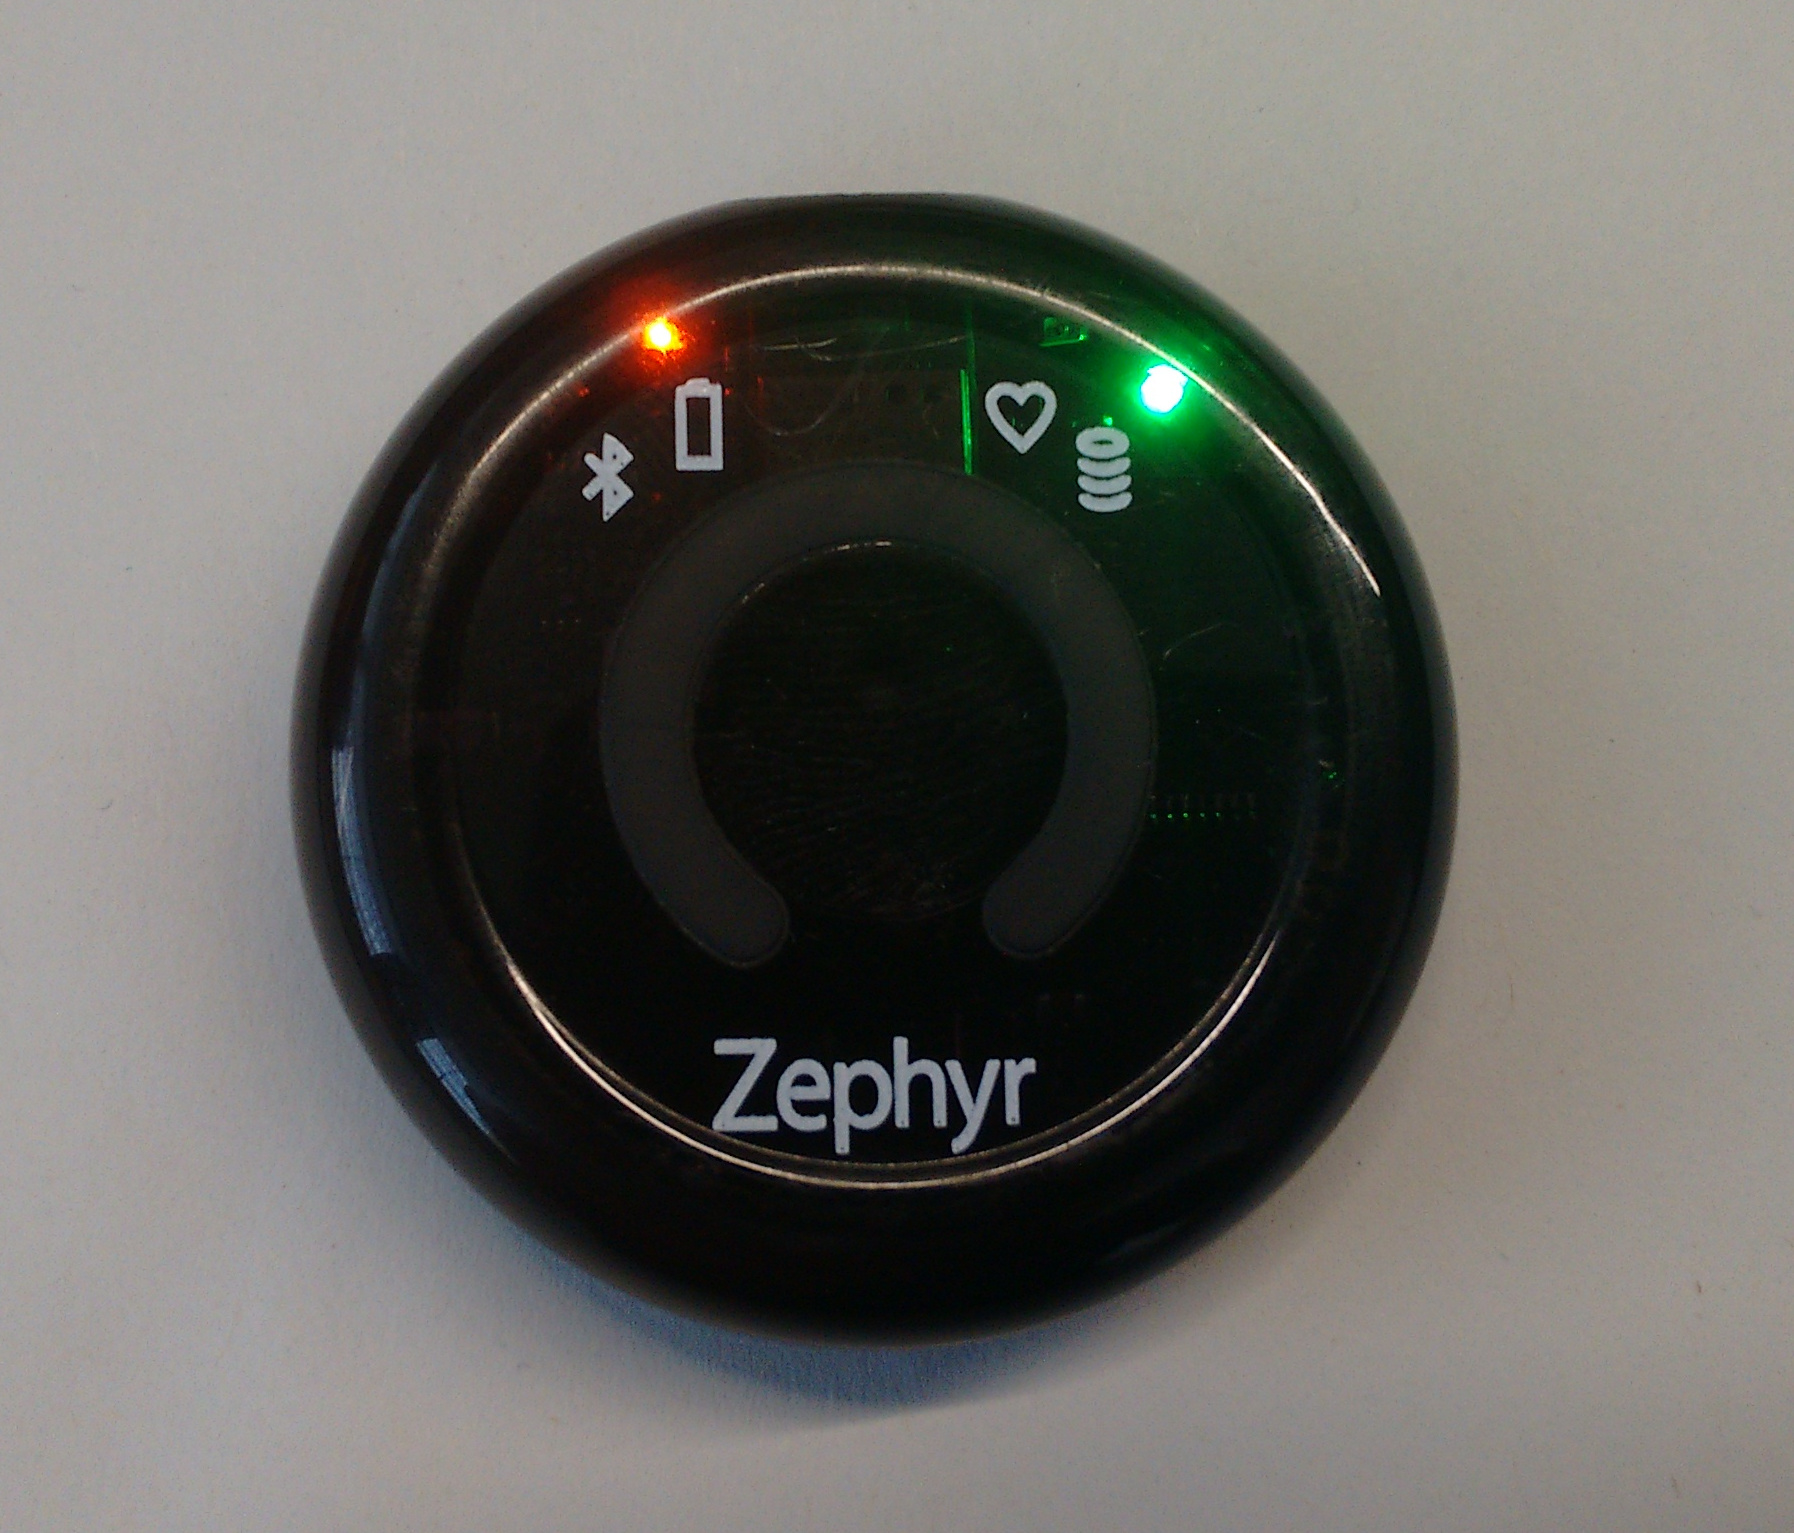
\includegraphics[width=0.5\textwidth]{./setup/zephyr}
\caption{Sesor Zephyr BioHarness 3}
%\label{a:arquitectura}
\end{center}
\end{figure}

El fabricante te ofrece gran cantidad de documentación y una aplicación de prueba para los desarrolladores que quieran realizar productos y utilicen sus sensores. Pero todo está orientado a aplicaciones Android, las cuales son las más populares para este tipo de sensores. 

Por lo tanto, después de buscar y ponerse en contacto con la empresa, no hay ningún tipo protocolo para establecer contacto y recibir los datos en JavaScript. Por lo que se decidió realizar uno utilizando toda la documentación y ejemplos para otros lenguajes. 

Para la realización del código de comunicación fueron necesarios 2 módulos de Node.js uno que nos calcula el CRC y otro que establece una conexión bluetooth.

Módulos utilizados:

\begin{itemize}
\item crc
\item bluetooth-serial-port 
\end{itemize}
\pagebreak

\subsection{Protocolo}

El código realizado para poder establecer la comunicaciones fue el siguiente:
 
Se cargan los módulos externos y se declaran las variables, la dirección MAC del sensor se pone a clavo para evitar interferencias con otros dispositivos bluetooth.

\begin{verbatim}
var crc = require('crc');
var btSerial = new (require('bluetooth-serial-port')).BluetoothSerialPort();

ADDRESS = "E0:D7:BA:A7:F1:5D";
var results = [];
var is_stopping = false;
\end{verbatim}

Función \texttt{connect}, como su nombre indica, nos conectara con el sensor y empezará a recibir datos. 

\begin{verbatim}
function connect(callback) {
   var socket = btSerial.on('found', function (address) {
       if (address == ADDRESS) {
           btSerial.findSerialPortChannel(address, function (channel) {
               btSerial.connect(address, channel, function () {
                   console.log('connected to ' + address);
                   btSerial.on('data', function (buffer) {
                       decode(buffer);
                   });
                   listener(socket, function (res) {
                       callback(res);
                   });
               }, function () {
                   console.log('cannot connect');
               });
           }, function () {
               console.log('found nothing');
           });
       }
   });
   btSerial.inquire();
}
\end{verbatim}

La función \texttt{decode}, nos permite decodificar de una manera muy simplificada los bytes que se reciben. Le pasa el segundo byte y según su valor se puede saber qué tipo de mensaje envía el sensor. Si en el segundo byte que se recibe es un 44 implica que en el noveno byte que se está recibiendo el ritmo cardiaco.

\begin{verbatim}
function decode(data) {
   switch (data[1]) {
       case 35:
           console.log("Received LifeSign message");
           break;
           \end{verbatim}
           %\pagebreak
           \begin{verbatim}
       case 44:
           console.log("Received Event message");
           results.push(data[8]);
           break;
       case 43:
           console.log("Received Summary Data Packet");
           break;
       case 37:
           console.log("Received Accelerometer Data Packet");
           break;
       case 36:
           console.log("Received R to R Data Packet");
           break;
       case 33:
           console.log("Received Breathing Data Packet");
           break;
       default:
           console.log("Packet type: " + data[1]);
           console.log("Received Not recognised message");
           break;
   }
}
\end{verbatim}

Una vez conectados al sensor se debe enviar mensajes a este para que mantenga la conexión y no se desconecte (\texttt{lifeSings}). Como la finalidad es realizar una medida la comunicación se realizará durante 20 seg, una vez pasados estos 20 seg se cerrara la conexion. 

\begin{verbatim}
function listener(socket, callback) {
   socket.on('data', function (buffer) {
       decode(buffer);
       lifeSing = create_message_frame('100011', 0);
       socket.write(new Buffer(lifeSing), function (err, bytesWritten) {
           if (err) console.log(err);
       });
   });
   setTimeout(function () {
       stop(socket, function (res) {
           callback(res);
       });
   }, 20000);
}
\end{verbatim}

La creación de los mensajes \texttt{lifeSings} se realizan de la siguiente manera: Son la concatenación de un byte de sincronismo, el mensaje, el dlc que será la longitud del payload, el crc calculado mediante el payload y por ultimo otro byte de cierre. Todo el paquete se pasará a hexadecimal y se procederá a enviarlo.
 \pagebreak
\begin{verbatim}
function create_message_frame(message_id, payload) {
   dlc = payload.toString().length;
   if (0 <= dlc <= 128) {
       crc_byte = crc.crc32(payload);
       message_bytes = '00000010'+ message_id + dlc + payload + crc_byte 
       + '00000011';
       message_fame = Bin2Hex(message_bytes);
       return message_fame
   }
}
\end{verbatim}

Por último la función de \texttt{stop} y la función de \texttt{avg}, la función de \texttt{stop} cerrará la conexión y la función de \texttt{avg} calcula la media de todas las medidas tomadas durante los 20 seg y devolverá la media. 

\begin{verbatim}
function stop(socket, callback) {
   is_stopping = true;
   socket.close();
   avg(function (res) {
       callback(res);
   });

}

function avg(callback) {
   var sum = 0;
   if (is_stopping == true) {
       for (var i = 0; i < results.length; i++) {
           sum = sum + results[i];
       }
       var media = sum / results.length;
       callback(media);
   }
}
\end{verbatim}

Con esto se puede establecer una conexión con el sensor y poder recibir la media del pulso cardiaco durante 20 seg. Hay que tener en cuenta la simplicidad del protocolo, ya que solo se captura una de las funciones (ritmo cardíaco) que proporciona el sensor Zephyr, ya que si se quiere obtener todos los datos la complejidad sería mucho mayor y para desarrollarlo en JavaScript se necesitaría mucha más información sobre cómo se envían las tramas y que contiene cada una de ellas.
\pagebreak
\section{Integración con Aaaida}

Como se explicó en el capítulo anterior la consola de Aaaida es una plataforma web, que nos permite administrar toda la información de las aplicaciones vinculadas a ella. 
Para poder incluir nuestra aplicación de monitorización del ritmo cardiaco con Aaaida y así visualizar lo en la web hay que crear un plugin de Aaaida con nuestro proyecto. 

\subsection{Creación de un plugin}

Para el desarrollo de cada uno de los plugins se ha utilizado el framework llamado route-injector desarrollado por Alteraid y Ondho. 

El objetivo principal de este framework es el de generar, de manera automática:
los método http CRUD de la API REST (GET, PUT, POST,DELETE) y una
backoffice, mediante modelos.

Para la creación del plugin de proyecto deberemos de seguir la arquitectura principal de los plugins.


\begin{figure}[htb]
\begin{center}
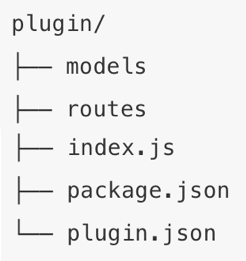
\includegraphics[width=0.35\textwidth]{./setup/arc}
\caption{Arquitectura de los plugins}
%\label{a:arquitectura}
\end{center}
\end{figure}

\subsubsection{Models}

En el caso de este proyecto no se creará ningún modelo de datos nuevo, ya que Aaaida dispone de un conjunto de modelos de datos que concuerda con el modelo que se necesita. El modelo elegido será Value, que cumple todas las necesidades de las medidas realizadas.

Los campos utilizados son los siguientes:

\begin{verbatim}
{
    value: {type: String},
    user: {type: mongoose.Schema.Types.Mixed, ref: 'User'},
    bond: {type: mongoose.Schema.Types.Mixed, ref: 'Bond'},
    measure: {type: mongoose.Schema.Types.Mixed, ref: 'Measure'},
    tags: {type: String},
    measured_at: {type: Date, readonly: true}
}
\end{verbatim}
\pagebreak

\begin{itemize}
\item value: Será el valor de la medida de ritmo cardiaco registrada. 
\item user: El usuario con el cual se está logueado en Aaaida
\item bond: Sería el “paciente” al cual se le toma la medida.
\item tags: Este campo se utiliza para diferenciar de qué aplicación pertenecen los valores.  
\item measured at: El instante que se tomó el valor. 
\end{itemize}

\subsubsection{Routes}

En el caso de que fuese necesario obtener información más concreta sobre el
modelo de datos, se deberían de definir cada una de esas rutas en la carpeta
routes del plugin. Como se dijo, route-injector genera automáticamente el CRUD para el modelo Values, pero necesita una ruta específica para ejecutar la conexión vía bluetooth con el sensor. 

Por lo tanto fue necesario la creación de la ruta, en el mismo fichero se copio todo el protocolo para la conexión con el sensor Zephyr. 

\begin{verbatim}
module.exports.route = function (router) {
   router.get('/coiote/media', function (req, res) {
       connect(function (media) {
           console.log("Tu HR media = " + media);
           res.json(media)
       });
   });
};
\end{verbatim}

Como se puede apreciar en el código una petición \texttt{get} a \texttt{ /coiote/media } ejecutará la función \texttt{connect} que establece la comunicación y recolección de datos.  

\subsubsection{Index}

En el siguiente fichero se configuran las funciones iniciales del plugin una vez
este ha cargado.

\begin{verbatim}
module.exports.config = require('./plugin.json');

module.exports.init = function (conf) { 
};
\end{verbatim}

El plugin no debe hacer ninguna función al iniciarse, por lo tanto, no debemos añadir nada en este fichero.
\pagebreak
\subsubsection{Package} 

En este fichero, se describe toda la información necesaria del paquete. 

\begin{verbatim}
{
 "name": "coiote-plugin",
 "version": "0.0.1",
 "description": "Plugin for CoIoTe",
 "dependencies": {
   "bluetooth-serial-port": "^2.0.0",
   "crc": "^3.4.0"
 }
}
\end{verbatim}

Se puede apreciar las 2 dependencias a módulos externos nombrados anteriormente. 

\subsubsection{Plugin} 

En este fichero, se indica el nombre del plugin y el directorio donde se encuentran
las rutas estáticas. Sirve para especificar dónde se encuentran todas esas rutas generadas para el plugin y no han sido creadas automáticamente por route-injector. 

\begin{verbatim}
{
 "name": "CoIoTe",
 "routes": ["routes"]
}
\end{verbatim}

\subsection{Creación de la página}

Una vez el plugin está creado, se necesitará crear la página web donde poder visualizar en la consola de Aaaida los resultados obtenidos de las medidas. 

Para esto se seguirá un proceso similar al de crear un plugin, pero en el directorio de \texttt{pages}, que tiene una arquitectura base similar a la siguiente:  

\begin{figure}[htb]
\begin{center}
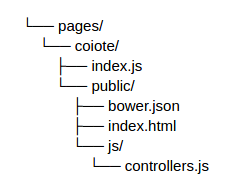
\includegraphics[width=0.35\textwidth]{./setup/arc2}
\caption{Arquitectura del directorio pages}
%\label{a:arquitectura}
\end{center}
\end{figure}


En este directorio, se encuentran definidos cada uno de los templates externos que se añadirán a la backoffice.

En este caso, ha sido necesario añadir el de coiote. En este directorio podemos encotrar el template index.js donde se define el controlador y como se visualiza en la consola de Aaaida y su URL. 

\begin{verbatim}
module.exports = {
   backoffice: true,
   url: 'coiote/mesures',
   template: 'coiote/index.html',
   controller: 'ChartCoioteController',
   menu: {
       clickTo: 'coiote/mesures',
       title: "mesures",
       section: "CoIoTe"
   }
   //backoffice: false // standalone website
};
\end{verbatim}

Creandonos una pestaña en la consola de Aaaida para el proyecto como podemos ver en la figura \ref{sec:coioteSec}. 

\begin{figure}[htb]
\begin{center}
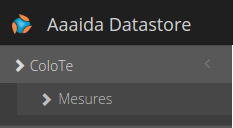
\includegraphics[width=0.25\textwidth]{./setup/arquitecturaCoiote}
\caption{Sección en la consola de Aaaida}
\label{sec:coioteSec}
\end{center}
\end{figure}

Una vez creado este fichero pasaremos a crear la template \texttt{index.html} y su controlador \texttt{controller.js}. En el controlador se realizan petición a las rutas creadas por route-injector para el modelo \texttt{value} y la ruta creada en el directorios \texttt{routes} para establecer la comunicación, y así poder rellenar el contenido de la plantilla.

La página para la visualización de los resultados sería esta:

\begin{figure}[htb]
\begin{center}
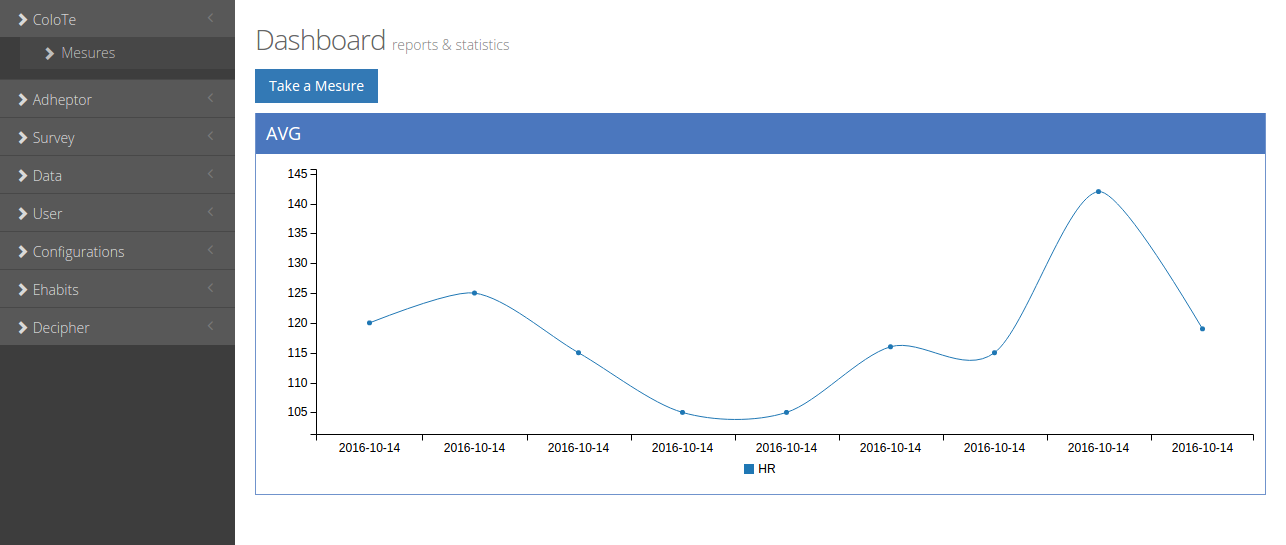
\includegraphics[width=1\textwidth]{./setup/visualizacionPaginaCoiote}
\caption{visualización de los datos en Aaaida}
%\label{sec:coioteSec}
\end{center}
\end{figure}
\pagebreak

\subsection{Recursos utilizados}

A continuación se mostrará en una tabla todos aquellos recursos de la API de Aaaida que fueron utilizados. 


\begin{table}[htb]

\begin{center}

\begin{tabular}{|c|c|c|}

\hline

{\bf Modelo} & {\bf Tipo} &

{\bf Ruta} \\ \hline \hline

Bond & get & /bond/:user.login  \\ \hline

Value & post & /values \\ \hline

Value & post & /value \\ \hline

- & get & /coiote/media \\ \hline

\end{tabular}

\caption{Exemple de taula}

\label{T:prova}

\end{center}

\end{table}

\begin{itemize}
\item Devuelve toda la información del usuario que está logueado en Aaaida.
\item Retorna los valores del bond del cual hemos tomado la medida.
\item Guarda el valor de la medida realizada. 
\item Establece la conexión y la recogida de datos.
\end{itemize}

\section{Despliegue en las Raspberry Pi}


\section{Conclusiones y Resultados}

Conseguir establecer la comunicación con el sensor fue una tarea para nada sencilla. Incluso haciendo tan solo la recogida de datos de una funcionalidad, se tuvo que entender muy bien cómo funcionaba y enviaba el sensor los datos. Sin contar que la documentación presentada por el fabricante se basaba únicamente en aplicaciones android. 

Como resultados, se desarrolló un protocolo de comunicación con el sensor, el cual nos proporcionaba la media  del ritmo cardiaco. La comunicación se podía ejecutar mediante la consola de Aaaida donde se visualizará el resultado y una vez validado se guardará en la base de datos. Para finalizar se proporciona una gráfica donde se puede ver un seguimiento de las medidas realizadas. 

\begin{figure}[htb]
\begin{center}
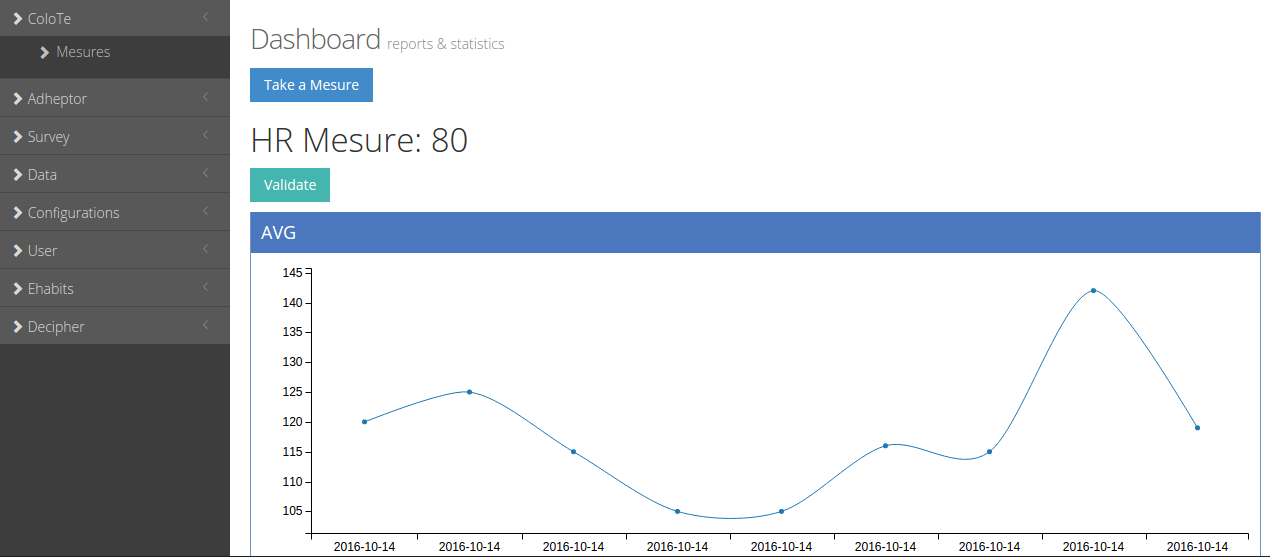
\includegraphics[width=1\textwidth]{./setup/final}
\caption{Consola de Aaaida}
%\label{sec:coioteSec}
\end{center}
\end{figure}
\pagebreak


